\chapter{Índices espectrales}

El objetivo de esta clase es la generación e intepretación de índices espectrales calculados a partir de bandas espectrales de \emph sentinel-2.


\section{Combinación color real}\label{sec:colorreal}

Abra la imagen \begin{center} \directory{S2B\_MSIL2A\_2018-01-31.dim}.
\end{center} seleccione \menu{Open RGB image windows} haciendo click derecho sobre el nombre de la imagen. Se desplegará una nueva ventana (Figura \ref{fig:RGB}) que le permitirá elegir la combinación de bandas. Por defecto aparecerá la combinación color real que utiliza las bandas \emph{rojo (B4)}, \emph{verde(B3)} y \emph{azul(B2)} de \emph{Sentinel-2}. Desplieguela haciendo click en \menu{OK}.

\section{NDVI}
El NDVI (Normalized Difference Vegetation Index) es uno de los índices más extendidos en teledetección. Utiliza la diferencia entre la absorción de la clorofila en el rojo y la reflectancia del infrarrojo cercano que se relaciona con la biomasa fotosintéticamente activa.

Para calcularlo, seleccione:

\begin{center}
\menu{Optical>Tematic Land Processing > Vegetation Radiometric Indices>NDVI Processor}
\end{center}

Se desplegará una nueva ventana (Figura \ref{fig:NDVI}). En \menu{Directory} seleccione la carpeta de salida para guardar el archivo en formato BEAM-DIMAP. Seleccione \menu {Run}. El producto ndvi se cargará en \menu{Product Explorer}. Para visualizarlo despliegue con doble click sobre el producto \menu {S2B\_MSIL2A\_2018-01-31>Bands} y seleccione \emph{ndvi}. En el visualizador se desplegará la imagen en escala de grises.

\begin{figure}[h!]
    \centering
    \subfloat[1-I/O Parameters]{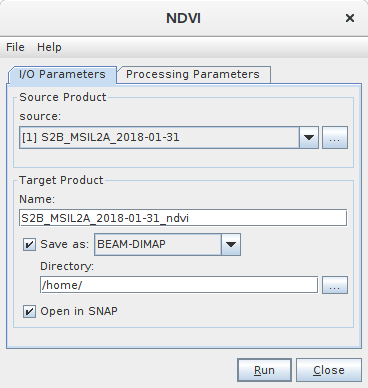
\includegraphics[width=0.4\textwidth]{fig:NDVI.png}\label{fig:NDVI}}
    \hspace{1cm}
    \subfloat[Processing parameters]{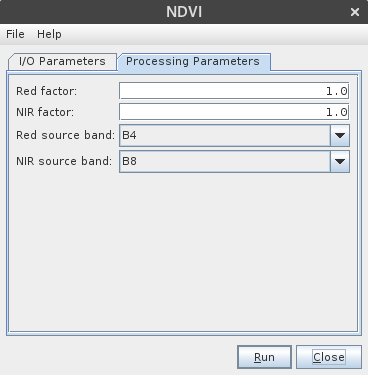
\includegraphics[width=0.4\textwidth]{fig:NDVI-par.png}\label{fig:NDVI-par}}
    \caption{Generacion del \emph{NDVI}.}
    \label{fig:NDVI}
\end{figure}

Identifique los diferentes usos y coberturas (Figura \ref{fig:mapa}) en el producto NDVI. Seleccione alguna cobertura y posicione el cursor en algún pixel de un parche homogéneo. Visualice el valor de \emph{NDVI} para ese parche. Para ello utilice la herramienta  \menu {pixel info}. Desplácece sobre la imagen con el cursor y visualice  los valores que toma el \emph{NDVI} para cada cobertura. Relacione estos valores con la escala de grises de la imagen.


\section{NDWI}

El NDWI (Normalized Difference Water Index) es un estimador del contenido de agua en el canopeo vegetal que interactua con la radación solar incidente. Es sensible a cambios en el contenido de agua en las hojas. Puede ser utilizado de manera complementaria al NDVI para monitoreo de contenido de agua y estado fisiológico en vegetación. Sin embargo es sensible al ruido del suelo sin cobertura.

Para calcularlo, seleccione \menu{Optical>Tematic Land Processing > Water Radiometric Indices>NDWI Processor}.  Se desplegará una nueva ventana (Figura \ref{fig:NDVI}). En \menu{Directory} seleccione la carpeta de salida para guardar el archivo en formato BEAM-DIMAP. Seleccione \menu {Run}. El producto \emph{NDWI} se cargará en \menu{Product Explorer}. Para visualizarlo despliegue con doble click sobre el producto \menu {S2B\_MSIL2A\_2018-01-31>Bands} y seleccione \emph{ndwi}. En el visualizador se desplegará la imagen en escala de grises. Compare y analice tal como lo hizo con el \emph{NDVI}

\section{SAVI}

El SAVI (Soil Adjusted Vegetation Index)  tal como el NDVI utiliza la diferencia entre la absorción de la clorofila en el rojo y la reflectancia del infrarrojo cercano. Tiene la ventaja de reducir el ruido de la reflectancia del suelo. Además permite ajustar el mismo de acuerdo al tipo de sustrato y porcentaje de cobertura. %re-redactar, está horrible.

Para calcularlo, seleccione \menu{Optical>Tematic Land Processing > Vegetation Radiometric Indices>SAVI Processor}.  Se desplegará una nueva ventana (Figura \ref{fig:NDVI}). En \menu{Directory} seleccione la carpeta de salida para guardar el archivo en formato BEAM-DIMAP. Seleccione \menu {Run}. El producto \emph{SAVI} se cargará en \menu{Product Explorer}. Para visualizarlo despliegue con doble click sobre el producto \menu {S2B\_MSIL2A\_2018-01-31>Bands} y seleccione \emph{savi}. En el visualizador se desplegará la imagen en escala de grises. Compare y analice tal como lo hizo con el \emph{NDVI}.

\section{Visualización con paleta de colores}

Una forma práctica de visualizar productos monobanda como el NDVI o SAVI es utilizando una paleta de colores mediante la cual puede observar los valores bajos con un determinado color, los valores intermedios con otro y así con los valores más altos, permitiendo además un gradiente de colores. %ver redacción

Seleccione en el \menu {Área de visualización} (Figura \ref{fig:color-man} el producto \emph{NDVI}. En \menu {Colour manipulation} podrá ver la distribución estadística de los pixeles del producto (Figura \ref{fig:color-man}). Seleccione la función \menu{import color palette from text file}. En el menú encontrará varias paletas de color,

seleccione  \directory{meris\_veg\_index}. En "Automatically distribuite points of colour palette between min/max?" seleccionar "Yes".

Se desplegará la imagen en tonos de verde, amarillo y naranja. Los valores NDVI altos se visualizarán en verde, en tanto que los valores intermedios en amarillo y los valores bajos en marrón oscuro. Relacione los valores con los colores observados (Figura \ref{fig:color-man-meris}).

Realice el mismo procedimiento para el \emph{SAVI}.

\begin{figure}[h!]
    \centering
    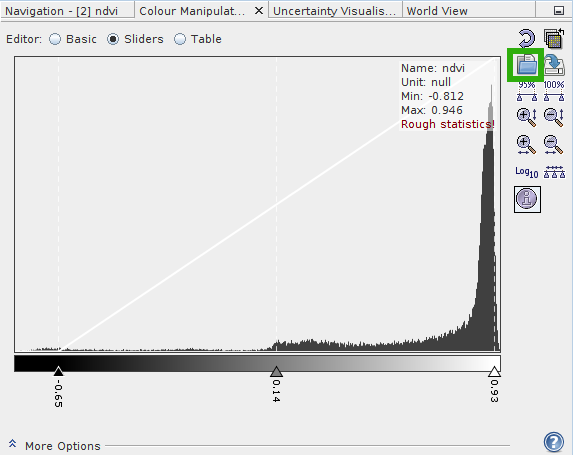
\includegraphics[width=0.6\textwidth]{fig:colour-man.png}
    \caption{Herramienta de Manipulación de Color. En sliders se observa la distribución estadístca de valores de NDVI}
    \label{fig:color-man}
\end{figure}

\begin{figure}[h!]
    \centering
    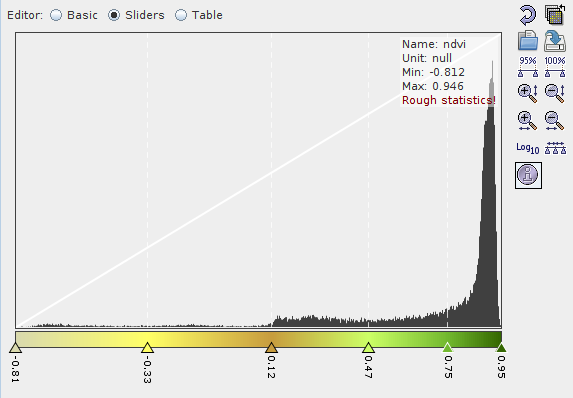
\includegraphics[width=0.6\textwidth]{fig:colour-man-meris.png}
    \caption{Herramienta de Manipulación de Color. En sliders se observa la distribución estadístca de valores de NDVI para la paleta de color meris.}
    \label{fig:color-man-meris}
\end{figure}

\section{Cálculo de estadísticas zonales}

En la práctica diaria es bastante común calcular las estadísticas básicas de un parche (e.g. media, varianza) para un conjunto de pixeles en lugar de un valor único. Para ello utilizaremos un conjunto de herramientas de análisis raster y vectorial.%ver redacción

En primer lugar crearemos polígonos para calcular sobre una parche las estadísticas para un determinado índice, por ejemplo NDVI.

\begin{enumerate}
\item Seleccione en \menu{Vector>New Vector Data Container}. Coloque el nombre del vector que corresponderá a una cobertura a estimar. Por ejemplo \emph{Selva Paranaense} (Figura \ref{fig:vector-container}).

\begin{figure}[h!]
    \centering
    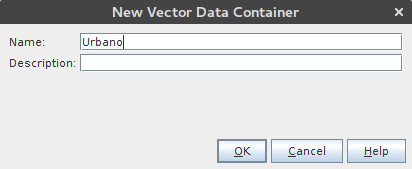
\includegraphics[width=0.6\textwidth]{fig:vector-cont.png}
    \caption{Herramienta Vector Container}
    \label{fig:vector-container}
\end{figure}


\item Repita el paso anterior para las coberturas \emph{sin cobertura vegetal} y \emph{cuerpo de agua}. Seleccione la herramienta \menu {Polygon Drawing Tool} (Figura xx). Se desplegará la ventana \menu{Select Vector Data Container}. Seleccione la cobertura correspondiente (e.g. Selva Paranaense). A continuación identifique el parche en el cual calculará las estadísticas y realice el polígono. De ese modo se generará un poligono correspondiente a ese uso y cobertura. Luego genere los vertices del polígono se haciendo click en la imagen. El cierre del polígono con dos clicks.

\begin{figure}[h!]
    \centering
    %\includegraphics[width=0.6\textwidth]{fig:}
    \caption{Herramienta Vector Container}
    \label{fig:vector-container}
\end{figure}

\item Cree el resto de los polígonos.
\end{enumerate}

%1 crear el vector container /va foto
% 2 poner los nombres de los usos y coberturas /va foto
% 3 generar los polígonos: 1 seleccionar selection tool, 2 seleccionar Polygon Drawning tool, 3  va foto
%






\section{Actividad práctica}
\begin{enumerate}
  \item Seleccione la imagen de NDVI aplicando la paleta de color \emph{meris}. Navegue con el cursor y obtenga el valor con la herramienta \menu {pixel info} para las siguientes coberturas.
  \begin{enumerate}

    \item Un parche homogéneo de selva paranaense que se observe en verde oscuro.
    \item Un parche homogéneo de selva paranaense que se observe en verde claro.
    \item Un parche hoomogéneo de suelo sin cobertura vegetal que se observa en marrón oscuro (cultivo en descanso).
    \item El embalse Urugua-í
    \item Vuelque los valores en una tabla y compare. ¿En qué tipo de coberturas encuentra los valores más altos? ¿Los más bajos? ¿Qué significado tiene los valores negativos?
    \item Grafique las firmas espectrales utilizando las herrramientas de la guía dos y analice para cada cobertura la relación entre infrarrojo cercano y rojo.
  \end{enumerate}


  \item Seleccione la imagen de SAVI aplicando la paleta de color \emph{meris} y repita el mismo procedimiento que para el NDVI.
  \begin{enumerate}
   \item Vuelque los valores en una tabla y compare. ¿En qué tipo de coberturas encuentra los valores más altos? ¿Los más bajos?
   \item Compare en la misma tabla los valores obtenidos para el NDVI.¿Cómo varían? ¿Son más altos o más bajos para SAVI? ¿Porqué?
 \end{enumerate}

\item Seleccione la imagen de NDWI aplicando la paleta de color \emph{meris} y repita el mismo procedimiento que para el NDVI.
  \begin{enumerate}
   \item Vuelque los valores en una tabla y compare. ¿En qué tipo de coberturas encuentra los valores más altos? ¿Los más bajos?
   \item Compare en la misma tabla los valores obtenidos para el NDVI.¿Cómo varían? ¿Son más altos o más bajos para SAVI? ¿Porqué?
  \end{enumerate}
\end{enumerate}

Estas preguntas y actividades no serán evaluadas. Su objetivo es discutirlas en el foro de consultas e intercambio de la clase.

%Comparar NDVI entre coberturas
%Comparar NDWI entre coberturas
%Comparar SAVI o GEMI
% Comparar la relacioon GEMI vs NDVI
% Hacer tabla comparativa entre indices


%Ver cómo manejar el tema de borrar pines en las comparaciones
% Añadir al anexo las longitudes de onda x mision satelital.
